% % % % % % % % % % % % % % % % % % % % % % % % % % % % % % % % % % % % % % % % % % % %
%                                                                                     %
% Short Sectioned Assignment LaTeX Template Version 1.0 (5/5/12)                      %
% This template has been downloaded from: http://www.LaTeXTemplates.com               %
%                                                                                     %
% Original author:  Frits Wenneker (http://www.howtotex.com)                          %
%                                                                                     %
% Modified by: Fco Javier Sueza Rodríguez (fcosueza@disroot.org)                      %
%                                                                                     %
% Changes:                                                                            %
%	    - Custom Chapters, Sections and Subsections (titlesec package)                %
%           - Document type scrbook (oneside)                                         %
%           - Use babel-lang-spanish package and marvosym                             %
%           - Use hyperref, enumitem, tcolorbox and glossaries packages               %
%           - Use Time New Roman (mathptmx), Helvetic and Courier fonts               %
%                                                                                     %
% License: CC BY-NC-SA 3.0 (http://creativecommons.org/licenses/by-nc-sa/3.0/)        %
%                                                                                     %
% % % % % % % % % % % % % % % % % % % % % % % % % % % % % % % % % % % % % % % % % % % %

%-----------------------------------------------%
%	              Packages                  %
%-----------------------------------------------%

\documentclass[paper=a4, fontsize=11pt, oneside]{scrbook}

% ---- Text Input/Output ----- %

\usepackage[T1]{fontenc}
\usepackage[utf8]{inputenc}
\usepackage{mathptmx}
\usepackage[scaled=.92]{helvet}
\usepackage{courier}
\usepackage[indent=12pt]{parskip}

\usepackage{geometry}
\geometry{verbose,tmargin=3cm,bmargin=3cm,lmargin=2.6cm,rmargin=2.6cm}

% ---- Language ----- %

\usepackage[spanish]{babel}
\usepackage{marvosym}

% ---- Another packages ---- %

\usepackage{amsmath,amsfonts,amsthm}
\usepackage{graphics,graphicx}
\usepackage{titlesec}
\usepackage{fancyhdr}
\usepackage{tcolorbox}
\usepackage{hyperref}
\usepackage{enumitem}
\usepackage[automake]{glossaries}

%--------------------------------------------------------------------%
%                      Customizing Document                          %
%--------------------------------------------------------------------%


% ----------- Custom Chapters, Sections and Subsections -------------- %

\titleformat{\chapter}[display]
			{\bfseries\Huge}
			{Tema \ \thechapter} {0.5ex}
			{\vspace{1ex}\centering}

\titleformat{\section}[hang]
			{\bfseries\Large}
			{\thesection}{0.5em}{}

\titleformat{\subsection}[hang]
			{\bfseries\large}
			{\thesubsection}{0.5em}{}

\titleformat{\subsubsection}[hang]
			{\bfseries\large}
			{\thesubsubsection}{0.5em}{}

\hypersetup{
    colorlinks=true,
    linkcolor=black,
    urlcolor=magenta
}

% ------------------- Custom heaaders and footers ------------------- %

\pagestyle{fancyplain}

\fancyhead[]{}
\fancyfoot[L]{}
\fancyfoot[C]{}
\fancyfoot[R]{\thepage}

\renewcommand{\headrulewidth}{0pt} % Remove header underlines
\renewcommand{\footrulewidth}{0pt} % Remove footer underlines

\setlength{\headheight}{13.6pt} % Customize the height of the header

% --------- Numbering equations, figures and tables ----------------- %

\numberwithin{equation}{section} % Number equations within sections
\numberwithin{figure}{section} % Number figures within sections
\numberwithin{table}{section} % Number tables within sections

% ------------------------ New Commands ----------------------------- %

\newcommand{\horrule}[1]{\rule{\linewidth}{#1}} % Create horizontal rule command


%----------------------------------------------------------------------------------------
%	TÍTULO Y DATOS DEL ALUMNO
%----------------------------------------------------------------------------------------

\title{
    \vspace{10ex}
    \normalfont \normalsize
    \huge \textbf{Actividades de la Unidad 2}
}
\author{Francisco Javier Sueza Rodríguez}
\date{\normalsize\today}

%----------------------------------------------------------------------------------------
%                                     DOCUMENTO
%----------------------------------------------------------------------------------------
\begin{document}

\maketitle

\thispagestyle{empty}

\vspace{75ex}

\begin{center}
    \begin{tabular}{l l}
        \textbf{Centro}: & IES Aguadulce \\
        \textbf{Ciclo Formativo}: & Desarrollo Aplicaciones Web (Distancia)\\
        \textbf{Asignatura}: & Entornos de Desarrollo\\
       \textbf{Tema}: & Tema 1 - Desarrollo de Software y Entornos de Desarrollo\\
    \end{tabular}
\end{center}

\newpage

\tableofcontents

\vspace{15ex}

\hrule

\vspace{10ex}

\listoffigures

\newpage

\section{Caso Práctico}
La empresa SOFTED ha recibido un nuevo encargo de software

En esta ocasión, todo el software que se desarrolle debería estar integrado en algún entorno de desarrollo libre. Ada ha elegido trabajar con NetBeans y utilizar como sistema operativo Windows o Linux.

Una vez planteado el análisis de requerimientos y el diseño de la aplicación (tal y como hicimos en la unidad anterior), se requiere tener un buen entorno para el diseño y ejecución de los programas.

- Venga, no te agobies, vamos a echar un café y nos ponemos manos a la obra,...- insiste Juan.

\section{Actividades}
En esta tarea vamos a realizar la instalación y configuración de \textbf{Netbeans 14}, así como ver un ejemplo de uso con una aplicación sencilla realizada en Java. Para esto, será también necesario la instalación del SDK de Java, en nuestro caso instalaremos la versión \textbf{JDK SE 11.0.13}, que realizaremos en primer lugar y antes de la instalación de Netbeans.

Además, en último lugar se instalará \textbf{Intellij IDEA}, para probar otro IDE a parte de Netbeans.

\subsection{Actividad 1}

\subsubsection{Enunciado}
Vamos a instalar el IDE Netbeans. Para ello se instalará por separado el JDK SE 11.0.13 y el IDE NetBeans 14. Puedes encontrar ambos archivos desde los enlaces del apartado 2.- Información de interés.

\begin{enumerate}[label=(\alph*)]
    \item Para la instalación de JDK cambia la carpeta de destino de instalación añadiendo una subcarpeta llamada XXX2223 (donde XXX sean tus iniciales), quedando la ruta: C:\textbackslash Program Files\textbackslash Java\textbackslash jdk-11.0.13\textbackslash XXX2223\ (para este apartado debes entregar dos capturas, la que muestra la carpeta de destino de la instalación con las modificaciones solicitadas y la captura de la última ventana que muestra que se ha finalizado la instalación correctamente).
    \item Para la instalación de Netbeans cambia la carpeta de destino de instalación añadiendo un subcarpeta llamada XXX2223 (donde XXX sean tus iniciales), quedando la ruta: C:\textbackslash Program File\textbackslash NetBeans-14\textbackslash XXX2223\ y el JDK instalado en el apartado anterior (para este apartado debes entregar otras dos capturas, la que se muestra en la carpeta de destino de la instalación con las modificaciones solicitadas y la captura de la última ventana que muestra que se ha finalizado la instalación correctamente).

    Capturas solicitadas: 4 (dos por cada apartado).
    \begin{itemize}
        \item Captura de pantalla donde se vea la instalación de JDK en la ruta indicada.
        \item Captura desde el símbolo del sistema donde se vea la versión instalada de JDK (para poder verlo escribimos en la consola: java -version)
        \item Captura mientras se instala NetBeans donde se vea la ruta de instalación indicada.
        \item Captura mostrando que el proceso de instalación ha finalizado correctamente.
    \end{itemize}
\end{enumerate}

\subsubsection{Solución}
En primer lugar vamos a instalar \textbf{JDK SE 13.0.11} y \textbf{Netbeans 14}. Hay que tener en cuenta que vamos a instalarlos \textbf{por separado} por lo que no nos vale el bundle que podemos encontrar donde Netbeans ya incluye el JDK en cuestión.

\begin{enumerate}[label=(\alph*)]
    \item Primeramente vamos a instalar el JDK solicitado. Para lo hemos descargarlo, desde \href{https://www.oracle.com/java/technologies/javase/jdk13-archive-downloads.html}{página oficial de Oracle} dedicada a las versiones antiguas. Una vez descargado ejecutamos el instalador y comenzamos el proceso de instalación. Nosotros hemos elegido como \textbf{directorio de instalación} la ruta \textbf{C:\textbackslash Program Files\textbackslash Java\textbackslash jdk-11.0.13\textbackslash FJS2223\ }, como se pide en el enunciado usando nuestras iniciales, como se puede ver en la siguiente captura.

    \begin{figure}[ht]
        \centering
        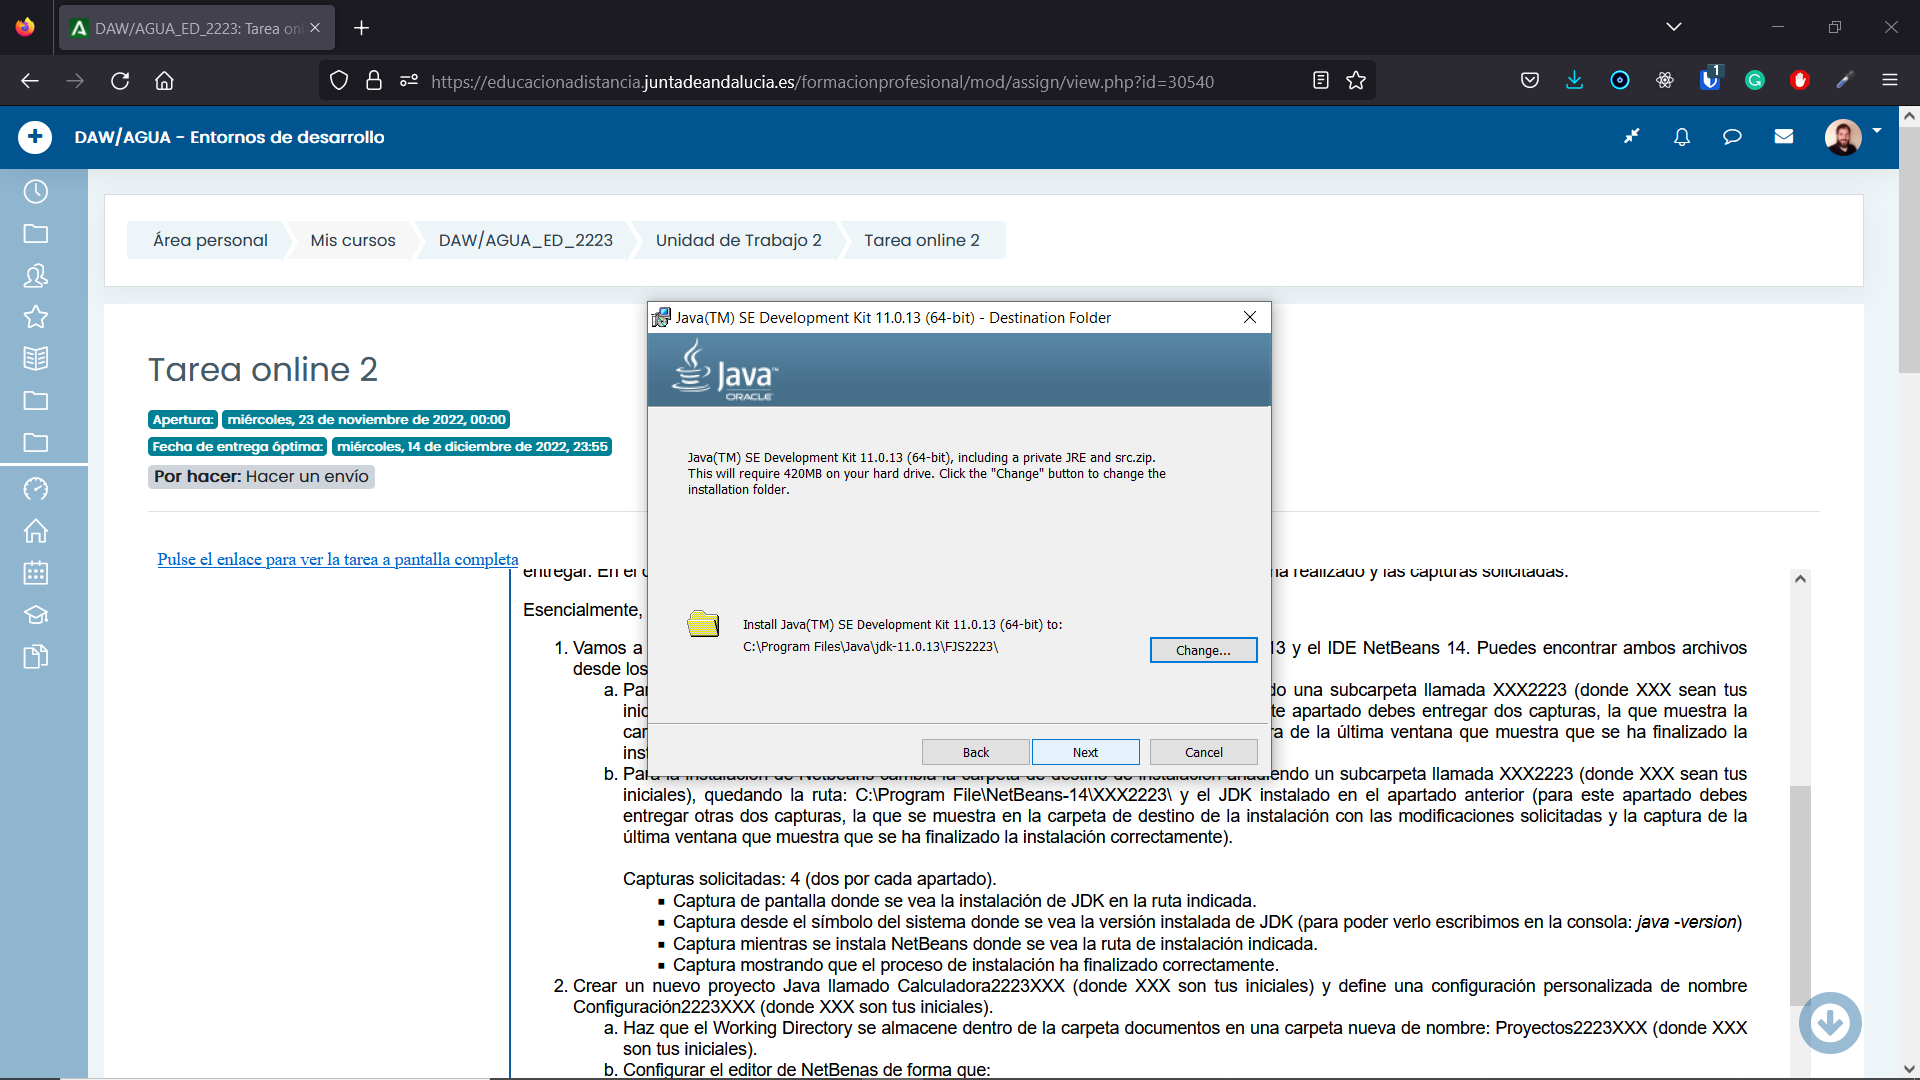
\includegraphics[scale=0.32]{jdk-install-1.png}
        \caption{Instalador de JDK y selección de directorio}
    \end{figure}

    Una vez seleccionado el directorio de instalación, ésta ha continuado con normalidad y se ha completado, como se muestra en la siguiente figura.

    \begin{figure}[ht]
        \centering
        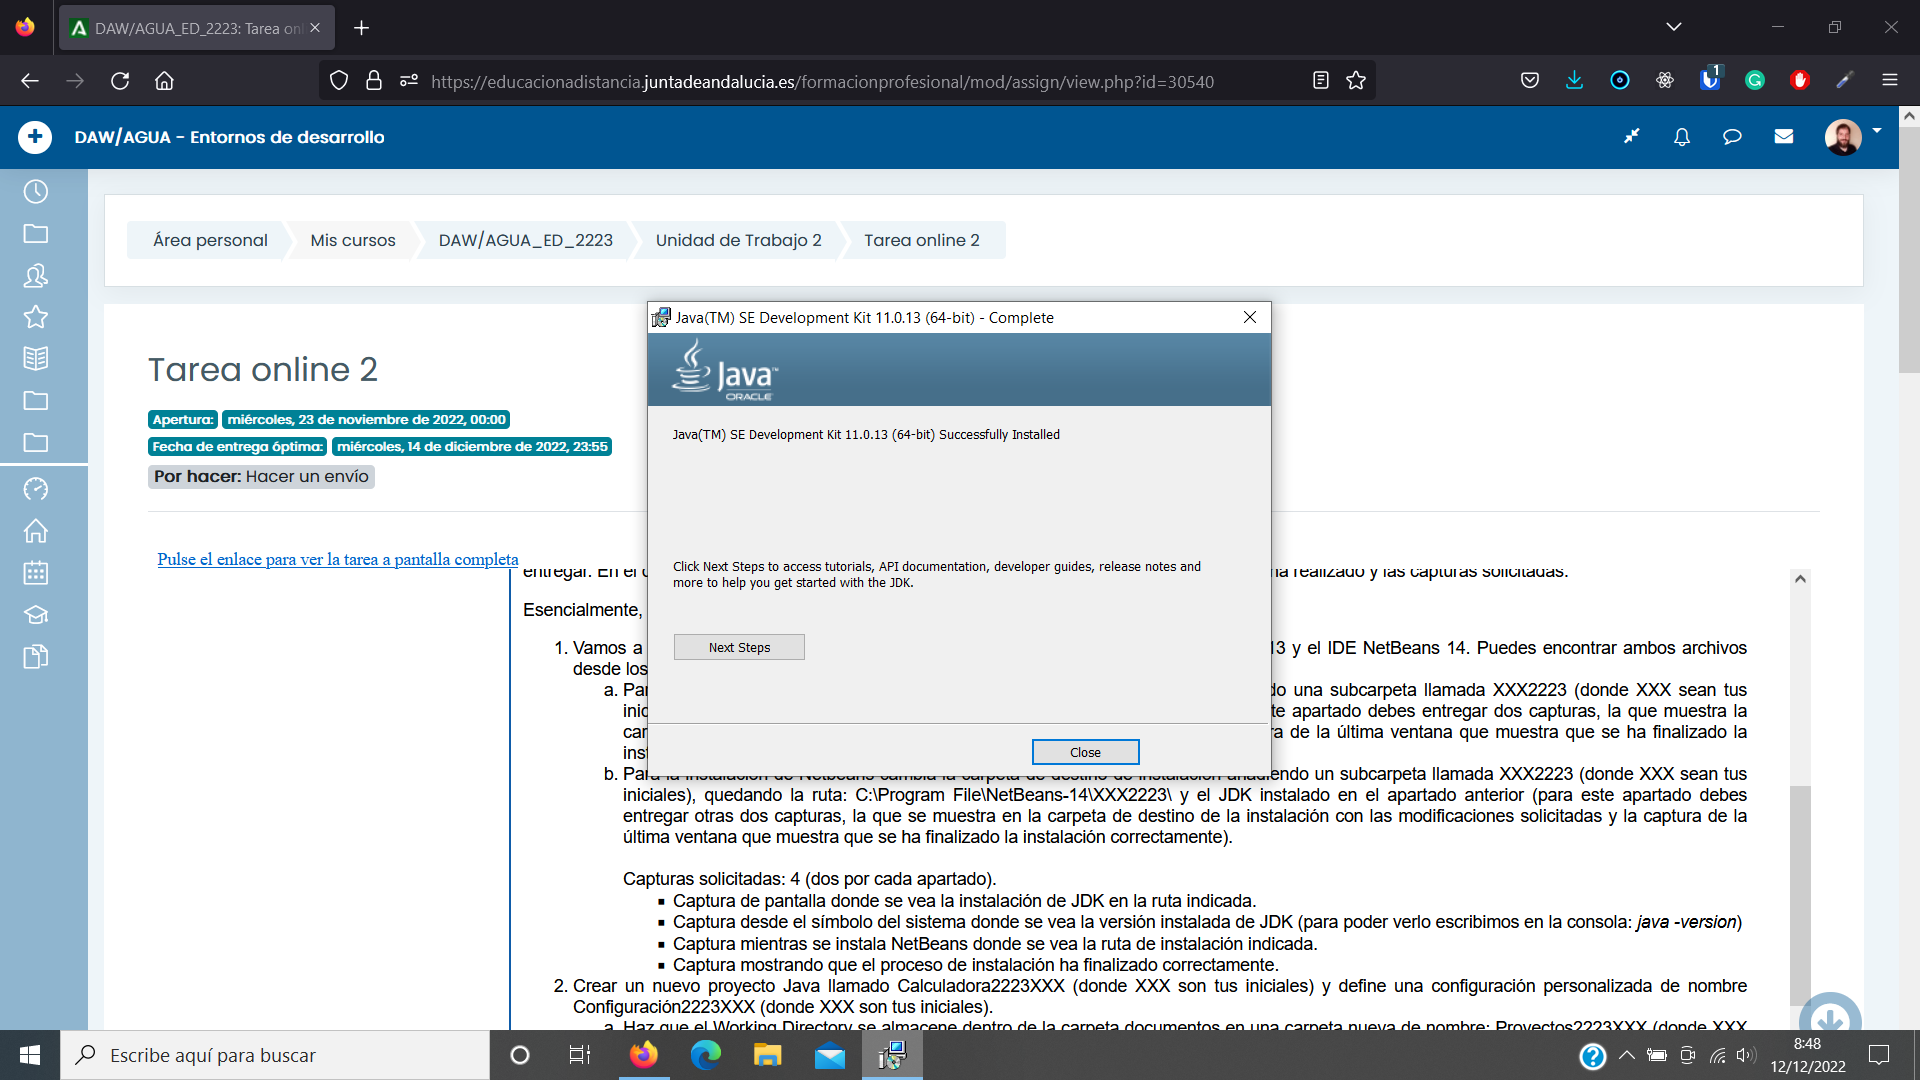
\includegraphics[scale=0.32]{jdk-install-2.png}
        \caption{Instalación de JDK SE completada}
    \end{figure}

    Para asegurarnos de que la instalación se ha realizado correctamente y la versión es la adecuada lo hemos comprobado desde la consola de Windows, usando el comando \textbf{``java --version''}.

    \begin{figure}[ht]
        \centering
        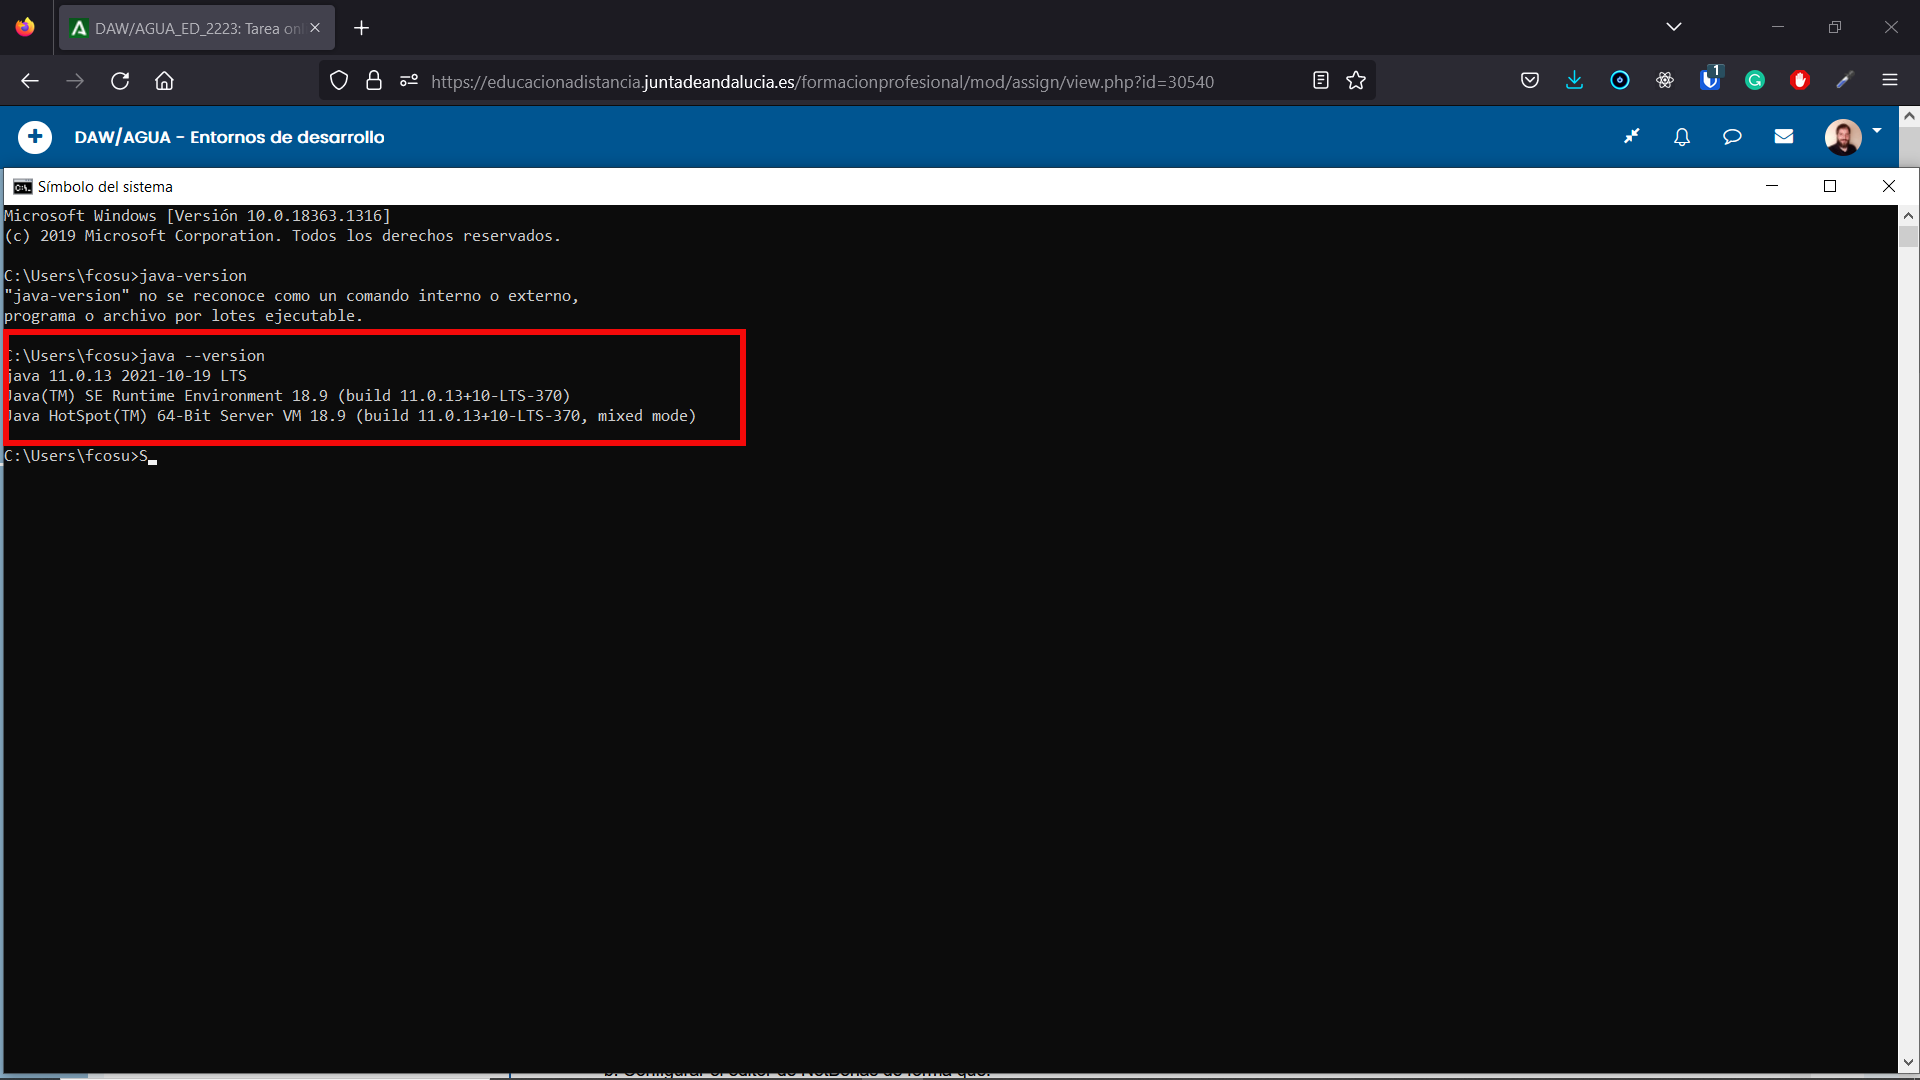
\includegraphics[scale=0.32]{jdk-install-3.png}
        \caption{Comprobación de versión de JDK instalada}
    \end{figure}

    \item A continuación hemos instalado \textbf{Netbeans 14}, descargando el instalador desde la \href{https://netbeans.apache.org/download/nb14/}{página oficial de netbeans}. Una vez ejecutado el instalador, se nos pide que seleccionemos los complementos a instalar, que nosotros hemos seleccionado por defecto. También se nos pedirá que especifiquemos la ruta del JDK instalado, aunque por norma general suele estar seleccionada la correcta por defecto.

     En la siguiente pantalla hemos cambiado el directorio de instalación al siguiente: \textbf{C:\textbackslash Program Files\textbackslash Netbeans-14\textbackslash FJS2223\ }.

    \begin{figure}[ht]
        \centering
        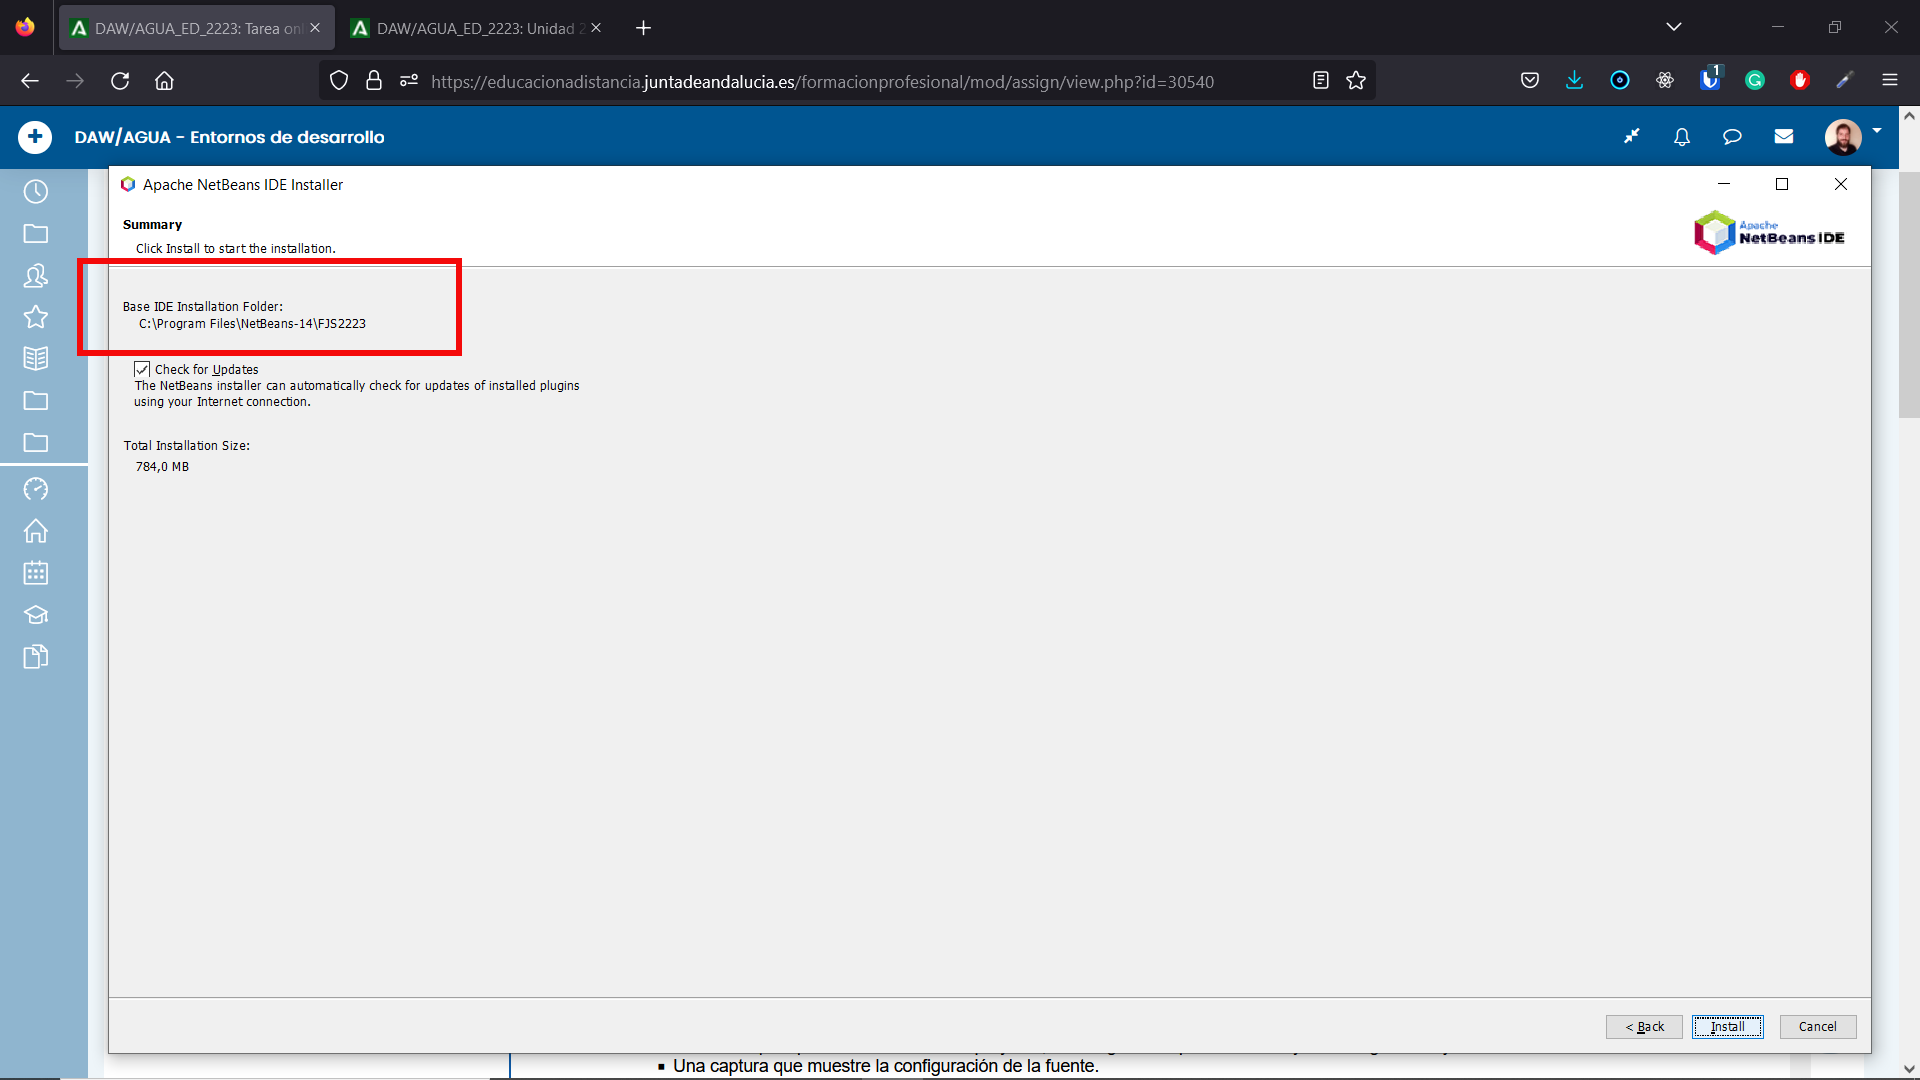
\includegraphics[scale=0.32]{netbeans-install-1.png}
        \caption{Instalador de Netbeans y selección de directorio}
    \end{figure}

    Después de seleccionar el directorio, hemos procedido con la instalación, la cual se ha realizado con éxito.

    \begin{figure}[ht]
        \centering
        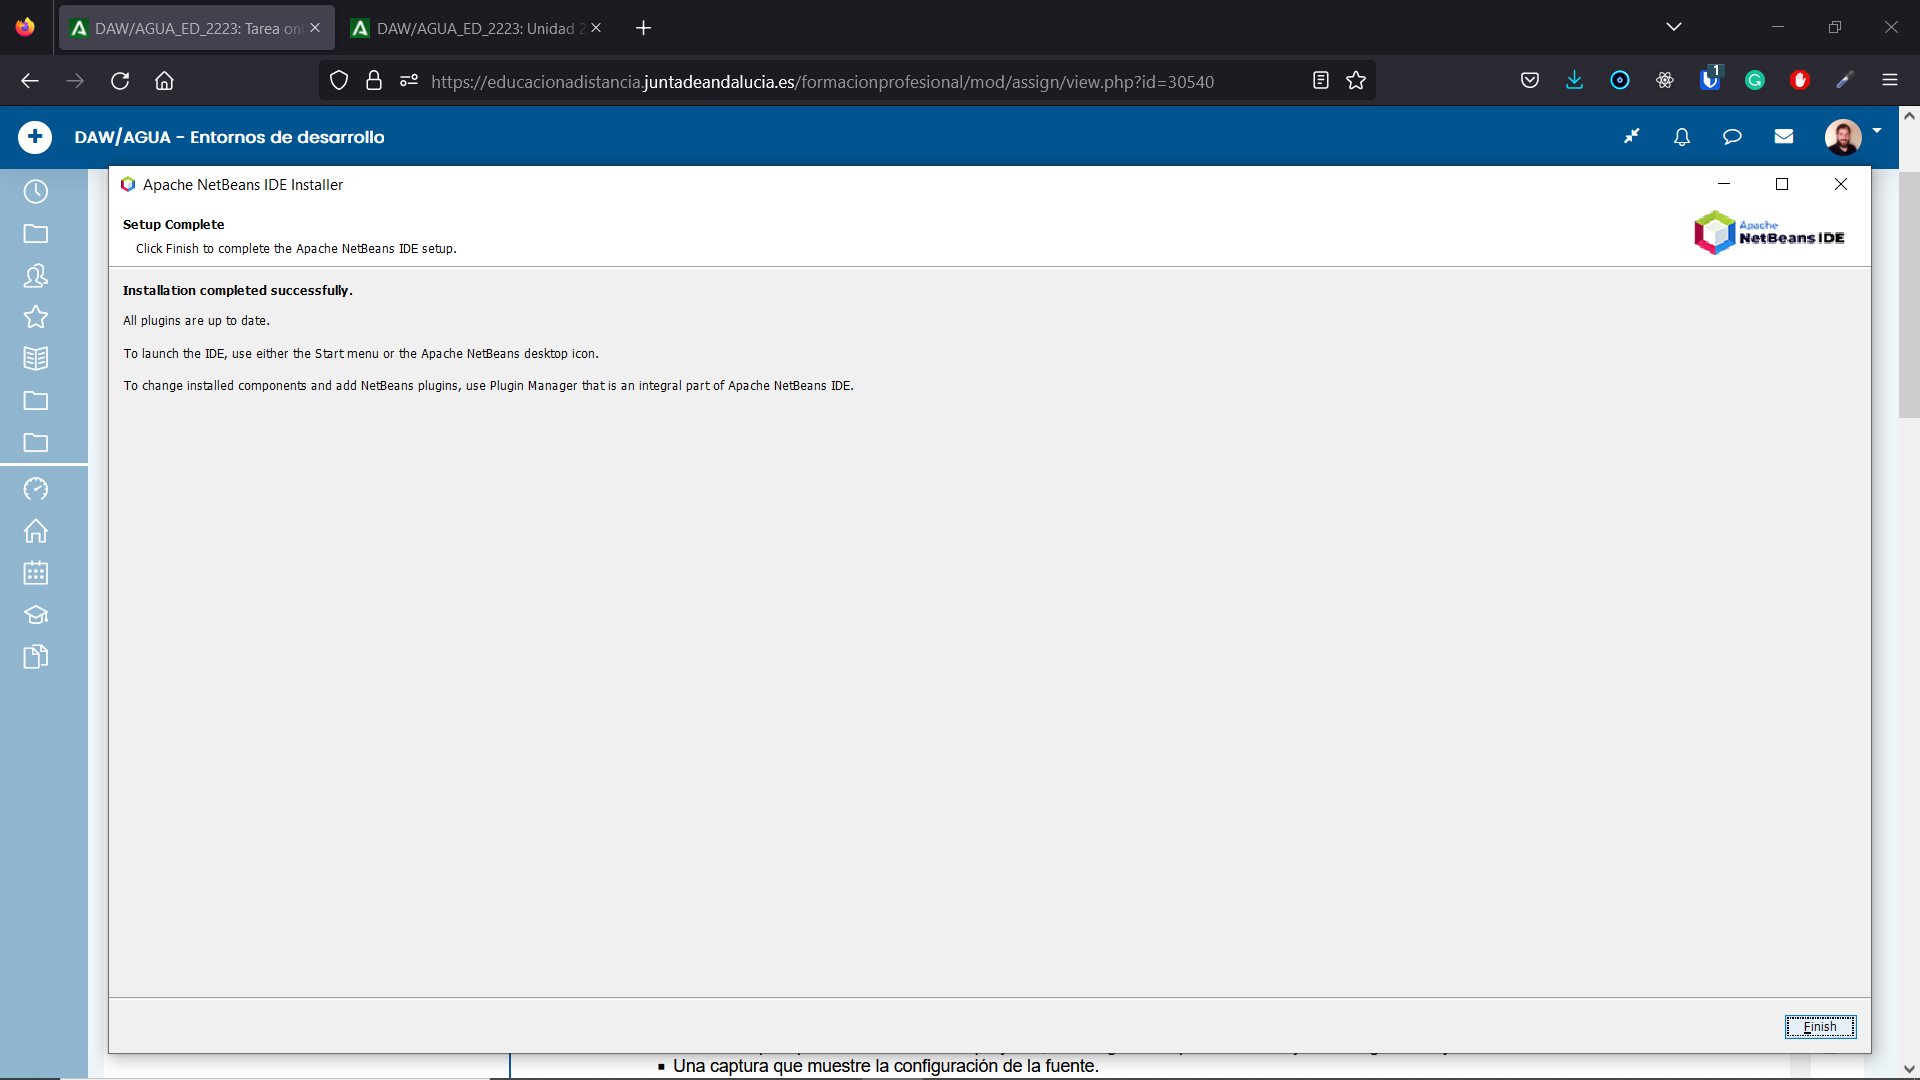
\includegraphics[scale=0.32]{netbeans-install-2.png}
        \caption{Instalación de Netbeans completada}
    \end{figure}
\end{enumerate}

\subsection{Actividad 2}
\subsubsection{Enunciado}
Crear un nuevo proyecto Java llamado Calculadora2223XXX (donde XXX son tus iniciales) y define una configuración personalizada de nombre Configuración2223XXX (donde XXX son tus iniciales).

\begin{enumerate}[label=(\alph*)]
    \item Haz que el Working Directory se almacene dentro de la carpeta documentos en una carpeta nueva de nombre: Proyectos2223XXX (donde XXX son tus iniciales).

    \item Configurar el editor de NetBenas de forma que:
    \begin{itemize}
        \item La fuente sea Arial 12 en azul
        \item Los Warning aparezcan con el texto en color naranja y negrita.
    \end{itemize}

    Capturas solicitadas: 3
    \begin{itemize}
        \item Una en la que aparezca el nombre del proyecto, la configuración personalizada y el woking directory.
        \item Una captura que muestre la configuración de la fuente.
        \item Una captura que muestre la configuración de los warning.
    \end{itemize}
\end{enumerate}

\subsubsection{Solución}








% Bibliography

\newpage
\bibliography{citas}
\bibliographystyle{unsrt}

\end{document}